\documentclass{article}
\usepackage{fontspec}
\usepackage{xeCJK}
\setCJKmainfont{Songti SC}
\setCJKsansfont{Heiti SC}
\setCJKmonofont{Songti SC}

\usepackage{amsmath, amssymb}
\usepackage{graphicx}
\usepackage{tikz}
\usepackage{hyperref}
\usepackage{geometry}
\usepackage{listings}
\usepackage{color}

\usetikzlibrary{automata, positioning, arrows}
\geometry{a4paper, margin=1in}

\title{编译原理作业 1}
\author{梁力航}
\date{\today}

\definecolor{dkgreen}{rgb}{0,0.6,0}
\definecolor{gray}{rgb}{0.5,0.5,0.5}
\definecolor{mauve}{rgb}{0.58,0,0.82}

\lstset{
    language=Python,
    aboveskip=3mm,
    belowskip=3mm,
    showstringspaces=false,
    columns=flexible,
    basicstyle={\small\ttfamily},
    numbers=left,
    numberstyle=\tiny\color{gray},
    keywordstyle=\color{blue},
    commentstyle=\color{dkgreen},
    stringstyle=\color{mauve},
    breaklines=true,
    breakatwhitespace=true,
    tabsize=3
}

\begin{document}

\maketitle

\section{作业 1}

\subsection{问题描述}
构造一个 DFA，接受所有在字母表 Sigma = {0,1} 上的字符串，满足以下条件：
不包含子串 "11"。

\subsection{解决方案}

\subsubsection{1. 正则表达式}

不包含 "11" 的字符串的正则表达式：
\begin{center}
$(0 | 10)^*(1 | \varepsilon)$
\end{center}

也可以简写为：
\begin{center}
$(0 | 10)^*1?$
\end{center}

\subsubsection{2. NFA 构造}

使用课程中教授的 Thompson 算法，从正则表达式 $(0 | 10)^*(1 | \varepsilon)$ 构造 NFA：

\begin{figure}[h]
    \centering
    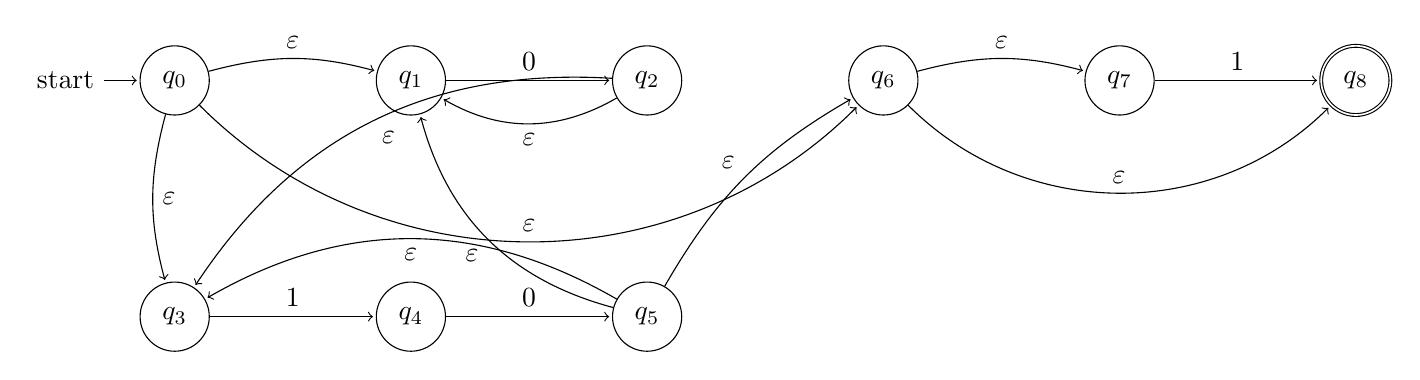
\begin{tikzpicture}[shorten >=1pt, node distance=3cm, on grid, auto]
        \node[state, initial] (q0) {$q_0$};
        \node[state] (q1) [right=of q0] {$q_1$};
        \node[state] (q2) [right=of q1] {$q_2$};
        \node[state] (q3) [below=of q0] {$q_3$};
        \node[state] (q4) [right=of q3] {$q_4$};
        \node[state] (q5) [right=of q4] {$q_5$};
        \node[state] (q6) [right=of q2] {$q_6$};
        \node[state] (q7) [right=of q6] {$q_7$};
        \node[state, accepting] (q8) [right=of q7] {$q_8$};
        
        \path[->]
        (q0) edge [bend left=15] node {\(\varepsilon\)} (q1)
        (q0) edge [bend right=15] node {\(\varepsilon\)} (q3)
        (q0) edge [bend right=45] node {\(\varepsilon\)} (q6)
        (q1) edge node {0} (q2)
        (q2) edge [bend left=30] node {\(\varepsilon\)} (q1)
        (q2) edge [bend right=30] node {\(\varepsilon\)} (q3)
        (q3) edge node {1} (q4)
        (q4) edge node {0} (q5)
        (q5) edge [bend left=30] node {\(\varepsilon\)} (q1)
        (q5) edge [bend right=30] node {\(\varepsilon\)} (q3)
        (q5) edge [bend left=15] node {\(\varepsilon\)} (q6)
        (q6) edge [bend left=15] node {\(\varepsilon\)} (q7)
        (q6) edge [bend right=45] node {\(\varepsilon\)} (q8)
        (q7) edge node {1} (q8);
    \end{tikzpicture}
    \caption{使用 Thompson 算法构造的不包含 "11" 的 NFA（含空串处理）}
    \label{fig:nfa}
\end{figure}

\paragraph{NFA 构造说明：}

1. \textbf{正则表达式分解}：$(0 | 10)^*(1 | \varepsilon)$
   - $A = 0$
   - $B = 10$
   - $C = 1$
   - $D = \varepsilon$
   - 整体是 $((A | B)^*)((C | D))$

2. \textbf{构造步骤}：
   - 为 $A=0$ 构造 NFA：$q_1 \xrightarrow{0} q_2$
   - 为 $B=10$ 构造 NFA：$q_3 \xrightarrow{1} q_4 \xrightarrow{0} q_5$
   - 为 $A|B$ 构造 NFA：添加起始状态 $q_0$，通过 ε-transition 连接到 $A$ 和 $B$ 的起始状态
   - 为 $(A|B)^*$ 构造 NFA：添加状态 $q_6$，通过 ε-transition 实现闭包操作
   - 为 $C=1$ 构造 NFA：$q_7 \xrightarrow{1} q_8$
   - 为 $D=\varepsilon$ 构造 NFA：$q_6 \xrightarrow{\varepsilon} q_8$
   - 为 $C|D$ 构造 NFA：通过 ε-transition 连接 $q_6$ 到 $q_7$ 和 $q_8$

3. \textbf{空串处理}：
   - 从起始状态 $q_0$ 到状态 $q_6$ 有直接的 ε-transition
   - 从状态 $q_6$ 到接受状态 $q_8$ 有直接的 ε-transition，确保空串被接受
   - 闭包操作的 ε-transition 也允许空串通过

\subsubsection{3. DFA 构造}

\begin{figure}[h]
    \centering
    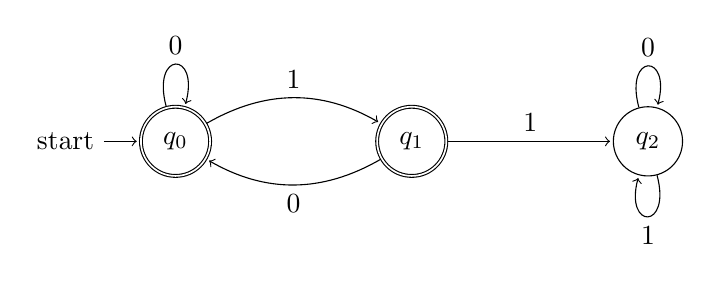
\begin{tikzpicture}[shorten >=1pt, node distance=3cm, on grid, auto]
        \node[state, initial, accepting] (q0) {$q_0$};
        \node[state, accepting] (q1) [right=of q0] {$q_1$};
        \node[state] (q2) [right=of q1] {$q_2$};
        
        \path[->]
        (q0) edge [loop above] node {0} (q0)
        (q0) edge [bend left=30] node {1} (q1)
        (q1) edge [bend left=30] node {0} (q0)
        (q1) edge node {1} (q2)
        (q2) edge [loop above] node {0} (q2)
        (q2) edge [loop below] node {1} (q2);
    \end{tikzpicture}
    \caption{不包含 "11" 的 DFA}
    \label{fig:dfa}
\end{figure}

\paragraph{DFA 转换表：}

\begin{center}
\begin{tabular}{|c|c|c|}
\hline
状态 & 输入 0 & 输入 1 \\
\hline
$q_0$ & $q_0$ & $q_1$ \\
$q_1$ & $q_0$ & $q_2$ \\
$q_2$ & $q_2$ & $q_2$ \\
\hline
\end{tabular}
\end{center}

\subsubsection{4. DFA 最小化}

上面的 DFA 已经是最小的。状态说明：

\begin{center}
\begin{tabular}{|c|c|c|}
\hline
状态 & 描述 & 接受 \\ 
\hline
$q_0$ & 未遇到 '1' 或最后一个字符是 '0' & 是 \\ 
$q_1$ & 最后一个字符是 '1' & 是 \\ 
$q_2$ & 包含 "11"（死状态） & 否 \\ 
\hline
\end{tabular}
\end{center}

\paragraph{最小化步骤：}

1. \textbf{初始划分}：分离接受和非接受状态
   - $P_0 = \{\{q_0, q_1\}, \{q_2\}\}$

2. \textbf{细化}：检查同一划分中的状态是否有相同的转换
   - 对于 $\{q_0, q_1\}$：
     - 输入 0：$q_0 \rightarrow q_0$，$q_1 \rightarrow q_1$（都停留在同一划分）
     - 输入 1：$q_0 \rightarrow q_1$，$q_1 \rightarrow q_2$（不同划分）
   - 因此，将 $\{q_0, q_1\}$ 划分为 $\{q_0\}$ 和 $\{q_1\}$

3. \textbf{最终划分}：$P_1 = \{\{q_0\}, \{q_1\}, \{q_2\}\}$

无法进一步划分，因此 DFA 是最小的，有 3 个状态。

\end{document}
